% ============================================================================== 
% Sat-Link manuscript prepared with the official MDPI LaTeX template
% Journal target: Telecom
% ============================================================================== 
% !TEX program = pdflatex
\documentclass[telecom,article,submit,pdftex,moreauthors]{Definitions/mdpi}

\firstpage{1}
\makeatletter
\setcounter{page}{\@firstpage}
\makeatother
\pubvolume{1}
\issuenum{1}
\articlenumber{0}
\pubyear{2026}
\copyrightyear{2026}
\datereceived{}
\daterevised{}
\dateaccepted{}
\datepublished{}

\usepackage{pgfplots}
\usepackage{lmodern}
\usepackage{siunitx}
\usepackage{flafter}
\pgfplotsset{compat=1.18}
\setlength{\headheight}{20pt}
\usetikzlibrary{shapes.geometric, arrows.meta, positioning, calc,
                fit, backgrounds, decorations.markings,
                patterns, shadows.blur}

% ── Colours used in TikZ diagrams ────────────────────────────────────
\definecolor{ieeblue}{HTML}{4F46E5}
\definecolor{ieepurple}{HTML}{7C3AED}
\definecolor{ieepink}{HTML}{EC4899}
\definecolor{ieeamber}{HTML}{F59E0B}
\definecolor{ieegreen}{HTML}{10B981}
\definecolor{blockbg}{HTML}{EEF2FF}
\definecolor{blockborder}{HTML}{6366F1}

% Compile safely even when external figure assets are not present in the workspace.
\newcommand{\mdpiincludegraphic}[2][]{%
  \IfFileExists{#2}{\includegraphics[#1]{#2}}{%
    \IfFileExists{#2.pdf}{\includegraphics[#1]{#2.pdf}}{%
      \IfFileExists{#2.png}{\includegraphics[#1]{#2.png}}{%
        \IfFileExists{#2.jpg}{\includegraphics[#1]{#2.jpg}}{%
          \IfFileExists{#2.jpeg}{\includegraphics[#1]{#2.jpeg}}{%
            \fbox{%
              \begin{minipage}[c][0.18\textheight][c]{0.9\linewidth}
                \centering
                Figure placeholder\\
                \texttt{#2}
              \end{minipage}%
            }%
          }%
        }%
      }%
    }%
  }%
}

\Title{Sat-Link: An Open-Source ITU-R-Based Satellite Link-Budget Simulator}

\Author{Nikolaos Kalaitzakis $^{1,*}$, Ioannis Papoudakis $^{1}$, Alexandros Kontos $^{1}$, Dimitrios Stratakis $^{1}$, Spyros Panagiotakis $^{1}$ and Manolis Tampouratzis $^{1}$}

\AuthorNames{Nikolaos Kalaitzakis, Ioannis Papoudakis, Alexandros Kontos, Dimitrios Stratakis, Spyros Panagiotakis and Manolis Tampouratzis}

\address{%
$^{1}$ \quad Department of Electrical and Computer Engineering, Hellenic Mediterranean University, Heraklion, Crete, Greece; th20458@edu.hmu.gr (N.K.); th20642@edu.hmu.gr (I.P.); th20308@edu.hmu.gr (A.K.); dstrat@hmu.gr (D.S.); spanag@hmu.gr (S.P.); tampouratzis@hmu.gr (M.T.)}

\corres{Correspondence: th20458@edu.hmu.gr (N.K.)}

\abstract{Satellite link-budget analysis is essential in both satellite-communication training and preliminary mission design. However, tools that seamlessly integrate orbital geometry, ITU-R propagation, and transponder characterization are still lacking in the field. This article introduces Sat-Link, the first open-source desktop simulator that performs end-to-end satellite link-budget analysis and preliminary trade-off studies. The simulator includes a model for free-space path loss, loss due to atmospheric gases, rain, clouds, and scintillation according to the ITU-R models, along with a model for Keplerian orbit propagation with J2 secular perturbations and user-defined drag. The modular design in Python/PyQt5 offers complete over budget, links, and transponder behavioral analyses, as well as interactive views of three-dimensional orbits and satellite constellations, user-defined parameter and statistical analyses, and pre-defined clickstream analyses of BER curves, ground track visualizations, and advanced analytics. The transponder chain models based on the Friis equation combined with noise cascading, and Saleh and Rapp models for high-power amplifier back-off and intermodulation, as well as the combined estimates of back-off and intermodulation effects. For representative GEO/Ku, LEO/S, and GEO/Ka scenarios, validation yielded a mean absolute error of 0.23 dB in Carrier-to-Noise Ratio over 0.30 dB deviation. Given these findings, Sat-Link can be used for educational purposes, but gamification and trade studies are not within the scope of the simulator.}

\keyword{satellite communications; link budget; ITU-R; propagation modeling; transponder nonlinearities; orbital mechanics; educational simulator}

\begin{document}

% ══════════════════════════════════════════════════════════════════════
%  I.  INTRODUCTION
% ══════════════════════════════════════════════════════════════════════
\section{Introduction}

Satellite link-budget analysis is one of the first topics taught in satellite communications and early mission design [1,2]. However, in teaching and workflow predesign, students and engineers have to make use of static spreadsheets and commercial software with low algorithmic transparency [3-5]. This combination makes it hard to explain design decisions regarding orbit, carrier frequency, coding and weather to the underlying physics and the associated standards models. Sat-Link is an open-source desktop tool that fills this gap. It combines interactivity with an ITU-R aligned uplink and downlink calculation, transponder nonlinearities, and orbit-dependent geometric effects into one software [6-14]. The simulator can model LEO, MEO, GEO, and HEO and can be used for real-time visual diagnostics and offline statistical analysis [15]. This work is focused on three primary contributions. First, Sat-Link offers a modular PyQt5 interface with seven view visualizations of complete link budgets, BER curves, constellation and ground track quality, 3D orbits, animated link and transponder behavior diagrams. Second, the software offers an ITU-R aligned link budget and transponder chain that combines cascading Friis noise with Saleh and Rapp HPA (Hot Pluggable) models and intermodulation noise. Third, it provides a reproducible benchmark test set and clearly defined scopes for pedagogical and pre-engineering design. The rest of the paper analyzes related software, discusses the software's architecture and associated mathematical models, summarizes the design of the user interface and workflow for advanced analysis and diagnostics, presents results of the validation and concludes with discussion on limitations and areas of use.
Overall, Sat-Link bridges theoretical link-budget analysis and practical system design by providing a transparent, reproducible, and ITU-R-aligned environment for education, early-stage satellite mission studies, and licensed amateur-radio experimentation.

% ══════════════════════════════════════════════════════════════════════
%  II.  RELATED WORK
% ══════════════════════════════════════════════════════════════════════
\section{Related Work}

Existing satellite-link tools span commercial platforms, numerical environments,
and astrodynamics libraries. Furthermore, measured studies show strong regional
sensitivity that makes transparent propagation modeling essential: for instance,
Usman \emph{et al.} reported 0.01\% rain attenuation ranging from 14--22~dB (Ku)
to 33--48~dB (Ka) depending on the elevation angle~\cite{usman2019_rain}.
Five representative tools highlight current gaps:

\begin{itemize}[leftmargin=*,nosep]
  \item \textbf{STK~\cite{ansys_stk}:} strong mission geometry, but
        communication-chain internals lack transparency for algorithm teaching.
  \item \textbf{MATLAB~\cite{mathworks_satcom}:} strong PHY experimentation,
        but complete ITU-R workflows require custom scripts in a commercial stack.
  \item \textbf{GMAT~\cite{nasa_gmat}:} open and reliable orbit design, but
        lacks integrated atmospheric and transponder link-budget workflows.
  \item \textbf{Orekit~\cite{orekit}:} excellent astrodynamics library, but
        leaves communication-specific GUIs and link-budget composition to the user.
  \item \textbf{ITU-Rpy~\cite{iturpy}:} a standalone Python library implementing
        the ITU-R P. series propagation algorithms, but provides no orbital
        mechanics, transponder modelling, or graphical user interface.
\end{itemize}


This comparison clarifies Sat-Link's design goal: not to replace high-end mission
suites, but to provide an auditable, standards-aligned, and classroom-ready
environment connecting orbit, propagation, and transponder effects in one workflow.

% ══════════════════════════════════════════════════════════════════════
%  III.  SOFTWARE ARCHITECTURE
% ══════════════════════════════════════════════════════════════════════
\section{Software Architecture}
\label{sec:architecture}


The simulator follows a model–view–controller (MVC) pattern implemented
in Python~3.9 with PyQt5 for the graphical front-end.  Fig.~\ref{fig:arch}
illustrates the layered design.

% ── TikZ: System Architecture Block Diagram ──────────────────────────
\begin{figure}[!t]
\centering
\begin{tikzpicture}[
    node distance=0.5cm and 0.4cm,
    block/.style={
        rectangle, draw=blockborder, fill=blockbg,
        rounded corners=3pt, minimum width=2.2cm,
        minimum height=0.7cm, font=\small\sffamily,
        text=black, align=center,
        blur shadow={shadow blur steps=3, shadow xshift=0.5pt,
                     shadow yshift=-0.5pt}
    },
    layer/.style={
        rectangle, draw=gray!60, dashed, rounded corners=5pt,
        inner sep=6pt, fill=white, fill opacity=0.3
    },
    arr/.style={-{Stealth[length=5pt]}, thick, ieeblue}
]
% --- Presentation Layer ---
\node[block, fill=ieepink!15, draw=ieepink!60] (header) {Header /\\Dashboard};
\node[block, fill=ieepink!15, draw=ieepink!60, right=of header] (tabs)
      {7 Viz Tabs};
\node[block, fill=ieepink!15, draw=ieepink!60, right=of tabs] (adv)
      {Advanced\\Analysis};
\node[layer, fit=(header)(tabs)(adv), label={[font=\footnotesize\sffamily,
      text=ieepink!80!black]above:Presentation Layer (PyQt5 / Matplotlib)}] (pres) {};

% --- Control Layer ---
\node[block, fill=ieeblue!15, draw=ieeblue!60, below=0.8cm of header]
      (ctrl) {Main Controller\\(\texttt{main\_advanced.py})};
\node[block, fill=ieeblue!15, draw=ieeblue!60, right=of ctrl]
      (hub) {Hub Manager};
\node[block, fill=ieeblue!15, draw=ieeblue!60, right=of hub]
      (export) {Export /\\PDF Engine};
\node[layer, fit=(ctrl)(hub)(export), label={[font=\footnotesize\sffamily,
      text=ieeblue!80!black]above:Controller Layer}] (ctl) {};

% --- Model Layer ---
\node[block, fill=ieegreen!15, draw=ieegreen!60, below=0.8cm of ctrl]
      (lb) {Link Budget\\(ITU-R)};
\node[block, fill=ieegreen!15, draw=ieegreen!60, right=of lb]
      (orb) {Orbit\\Mechanics};
\node[block, fill=ieegreen!15, draw=ieegreen!60, right=of orb]
      (mod) {Modulation\\/ Coding};
\node[block, fill=ieeamber!15, draw=ieeamber!60, below=0.5cm of lb]
      (tp) {Transponder\\Model};
\node[block, fill=ieeamber!15, draw=ieeamber!60, right=of tp]
      (bp) {Beam\\Pattern};
\node[block, fill=ieeamber!15, draw=ieeamber!60, right=of bp]
      (const) {Constants\\(ITU-R)};
\node[layer, fit=(lb)(orb)(mod)(tp)(bp)(const),
      label={[font=\footnotesize\sffamily, text=ieegreen!70!black]above:
      Model Layer (Physics / Standards)}] (mdl) {};

% --- Arrows ---
\draw[arr] (tabs.south) -- (ctrl.north);
\draw[arr] (header.south) -- (ctrl.north);
\draw[arr] (adv.south) -- (export.north);
\draw[arr] (ctrl.south) -- (lb.north);
\draw[arr] (hub.south) -- (orb.north);
\draw[arr] (export.south) -- (mod.north);
\draw[arr] (lb.south) -- (tp.north);
\draw[arr] (orb.south) -- (bp.north);
\draw[arr] (mod.south) -- (const.north);
\end{tikzpicture}
\caption{Three-layer simulator architecture: presentation, controller,
  and model layers.}
\label{fig:arch}
\end{figure}

\subsection{Module Organisation}

The implementation now follows the current repository layout:
\begin{itemize}[leftmargin=*,nosep]
  \item \texttt{main\_advanced.py}: main desktop entry point.
  \item \texttt{models/}: link budget, orbit, modulation, beam pattern,
        satellite, transponder, and constants modules.
  \item \texttt{gui/visualizations/}: seven primary tab views
        (link budget, BER, constellation, ground track, 3D view,
        link diagram, transponder).
  \item \texttt{gui/advanced\_analysis/}: advanced analysis dialog.
  \item \texttt{gui/hub/}, \texttt{gui/panels/}, \texttt{gui/dialogs/},
        \texttt{gui/core/}: hub management, header/dashboard panels,
        dialogs, and shared UI/splash/canvas components.
  \item \texttt{gui/utils/}: export, preset, and save/load utilities.
  \item \texttt{assets/} and \texttt{txt\_info/}: static resources and
        bundled reference text files.
  \item \texttt{requirements.txt}, \texttt{install.ps1},
        \texttt{run\_advanced.ps1}: dependency and Windows setup/run scripts.
\end{itemize}

Dependencies include PyQt5/PyQtWebEngine, NumPy, SciPy, Matplotlib,
pyqtgraph, Plotly, Pandas, Seaborn, and optional PyVista/PyVistaQt for
3D rendering, with Skyfield/SGP4/pyorbital for orbital workflows.
All ITU-R propagation models used in Sat-Link (P.525, P.618, P.676, P.838, P.840) were implemented independently from the original ITU-R Recommendations; the external ITU-Rpy library~\cite{iturpy} was not used in the computation chain, although it remains a useful independent reference implementation of the ITU-R P-series algorithms.

% ══════════════════════════════════════════════════════════════════════
%  III.  MATHEMATICAL MODELS
% ══════════════════════════════════════════════════════════════════════
\section{Mathematical Models}
\label{sec:models}

\subsection{Link-Budget Chain}

The complete link budget follows the cascaded carrier-to-noise methodology
of ITU-R~S.1328~\cite{itu_s1328}.  Each link direction (uplink and
downlink) is computed independently, then combined at the transponder
output.  The key expressions are summarised below.

\subsubsection{Free-Space Path Loss (ITU-R P.525)}
\begin{equation}
  \text{FSPL}~[\text{dB}] = 20\log_{10}(d) + 20\log_{10}(f) + 92.45
  \label{eq:fspl}
\end{equation}
where $d$ is the slant range in~km and $f$ the carrier frequency in~GHz.

\subsubsection{Rain Attenuation (ITU-R P.838-3 / P.618-14)}
The specific attenuation $\gamma_R$ is:
\begin{equation}
  \gamma_R = k\,R^{\alpha} \quad [\text{dB/km}]
  \label{eq:rain_specific}
\end{equation}
where $R$ is the rain rate in~mm/h and the coefficients $(k,\alpha)$ are
frequency- and polarisation-dependent as tabulated in
ITU-R~P.838-3~\cite{itu_p838}.  The total rain attenuation is:
\begin{equation}
  A_{\text{rain}} = \gamma_R \cdot L_s \cdot r
  \label{eq:rain_total}
\end{equation}
with $L_s$ the effective slant path length and $r$ a reduction factor
per~\cite{itu_p618}.

\subsubsection{Gaseous Attenuation (ITU-R P.676-12)}
Oxygen and water-vapour absorption are modelled as:
\begin{equation}
  A_{\text{atm}} = \frac{\gamma_o\,h_o + \gamma_w\,h_w}{\sin E}
  \label{eq:gas}
\end{equation}
where $\gamma_o$, $\gamma_w$ are specific attenuations, $h_o \approx
\SI{6}{km}$, $h_w \approx \SI{2}{km}$ the equivalent heights, and $E$
the elevation angle \cite{itu_p676}.

\subsubsection{Cloud Attenuation (ITU-R P.840-8)}
Cloud and fog attenuation is computed from the integrated liquid water
content~$L$ (kg/m$^2$) and a frequency-dependent specific attenuation
coefficient~$K_l$:
\begin{equation}
  A_{\text{cloud}} = \frac{K_l \cdot L}{\sin E}
  \quad [\text{dB}]
  \label{eq:cloud}
\end{equation}
where $K_l$ depends on frequency and temperature per the Rayleigh
scattering model \cite{itu_p840}.

\subsubsection{Tropospheric Scintillation (ITU-R P.618-14)}
Amplitude scintillation is characterised by its standard deviation:
\begin{equation}
  \sigma_{\text{scint}} = \sigma_{\text{ref}} \cdot f^{0.45}
    \cdot \frac{g(x)}{(\sin E)^{1.3}}
  \label{eq:scint}
\end{equation}
where $\sigma_{\text{ref}}$ is a reference deviation dependent on
$N_{\text{wet}}$ (wet-term refractivity), $f$ the frequency in~GHz,
and $g(x)$ an antenna-averaging function.  The fade depth exceeded for
a time percentage~$p$ is then $A_s(p) = a(p)\,\sigma_{\text{scint}}$.
In the current implementation, operational plots use the common
$p=0.01\%$ approximation $A_s \approx 2.6\,\sigma_{\text{scint}}$.

\subsubsection{Slant Range Geometry}
The Earth--satellite slant range $d$ relates to the elevation angle~$E$
and satellite altitude~$h$ above the Earth's surface:
\begin{equation}
  d = R_E\!\left[\sqrt{\left(\frac{R_E + h}{R_E}\right)^{\!2}
      - \cos^2\!E\,} - \sin E\right]
  \label{eq:slant}
\end{equation}
where $R_E = \SI{6371}{km}$ is the mean Earth radius.  This expression
is used in both the FSPL and the atmospheric path-length calculations.

\subsubsection{Carrier-to-Noise Density Ratio}
\begin{equation}
  \frac{C}{N_0} = \text{EIRP} - \text{FSPL} - A_{\text{total}}
                  + \frac{G}{T} - k_B
  \label{eq:cn0}
\end{equation}
with $k_B = -228.6$\,dBW/K/Hz the Boltzmann constant.

\subsubsection{Total System \texorpdfstring{$C/N_0$}{C/N0} (ITU-R S.1328)}
The total system performance combines uplink, downlink, and
intermodulation:
\begin{equation}
  \left(\frac{C}{N_0}\right)_{\!\text{total}}^{\!-1}
  = \left(\frac{C}{N_0}\right)_{\!\text{up}}^{\!-1}
  + \left(\frac{C}{N_0}\right)_{\!\text{dn}}^{\!-1}
  + \left(\frac{C}{IM_0}\right)^{\!-1}
  \label{eq:total_cn0}
\end{equation}

% ── TikZ: Link Budget Flow Diagram ──────────────────────────────────
\begin{figure}[!t]
\centering
\begin{tikzpicture}[
    node distance=0.35cm,
    step/.style={
        rectangle, draw=ieeblue!70, fill=ieeblue!8,
        rounded corners=2pt, minimum width=3.4cm,
        minimum height=0.55cm, font=\footnotesize\sffamily,
        align=center
    },
    result/.style={
        rectangle, draw=ieegreen!70, fill=ieegreen!10,
        rounded corners=2pt, minimum width=3.4cm,
        minimum height=0.55cm, font=\footnotesize\sffamily\bfseries,
        align=center
    },
    arr/.style={-{Stealth[length=4pt]}, thick, gray!70}
]
\node[step={}] (eirp) {EIRP = $P_{tx}$ + $G_{tx}$};
\node[step={}, below=of eirp] (fspl) {FSPL (P.525)};
\node[step={}, below=of fspl] (gas)  {Gas Atten. (P.676)};
\node[step={}, below=of gas]  (rain) {Rain Atten. (P.838)};
\node[step={}, below=of rain] (cloud){Cloud Atten. (P.840)};
\node[step={}, below=of cloud](scint){Scintillation (P.618)};
\node[step={}, below=of scint](gt)   {$G/T$ (Receiver)};
\node[result, below=of gt] (cn0)  {$C/N_0$ (dB-Hz)};
\node[result, below=of cn0](margin){Link Margin (dB)};

\foreach \a/\b in {eirp/fspl, fspl/gas, gas/rain, rain/cloud,
                   cloud/scint, scint/gt, gt/cn0, cn0/margin}
  \draw[arr] (\a) -- (\b);
\end{tikzpicture}
\caption{Sequential computation flow of a single-link budget.
  Each step implements the referenced ITU-R Recommendation.}
\label{fig:linkflow}
\end{figure}

\subsection{Transponder Model}

The satellite transponder is modelled as a four-stage cascaded chain
(Fig.~\ref{fig:transponder}): low-noise amplifier (LNA), mixer,
intermediate-frequency amplifier (IF~Amp), and power amplifier (PA/HPA).

% ── TikZ: Transponder Chain ──────────────────────────────────────────
\begin{figure}[!t]
\centering
\begin{tikzpicture}[
    node distance=0.15cm,
    stage/.style={
        rectangle, draw=blockborder, fill=blockbg,
        rounded corners=2pt, minimum width=1.6cm,
        minimum height=1.0cm, font=\footnotesize\sffamily,
        align=center
    },
    arr/.style={-{Stealth[length=5pt]}, thick, ieeblue},
    lbl/.style={font=\tiny\sffamily, text=gray!70!black}
]
\node (in) {\footnotesize $f_1$};
\node[stage, right=0.35cm of in]   (lna) {LNA\\{\tiny$G$=30\,dB}\\{\tiny NF=1.2\,dB}};
\node[stage, right=of lna]  (mix) {Mixer\\{\tiny$G$=-6\,dB}\\{\tiny NF=8\,dB}};
\node[stage, right=of mix]  (ifa) {IF Amp\\{\tiny$G$=35\,dB}\\{\tiny NF=4\,dB}};
\node[stage, right=of ifa]  (hpa) {HPA\\{\tiny$G$=15\,dB}\\{\tiny P\textsubscript{sat}}};
\node[right=0.35cm of hpa]  (out) {\footnotesize $f_2$};

\draw[arr] (in) -- (lna);
\draw[arr] (lna) -- (mix);
\draw[arr] (mix) -- (ifa);
\draw[arr] (ifa) -- (hpa);
\draw[arr] (hpa) -- (out);

\node[lbl, above=0.15cm of lna] {$T_1$};
\node[lbl, above=0.15cm of mix] {$T_2/G_1$};
\node[lbl, above=0.15cm of ifa] {$T_3/(G_1 G_2)$};
\node[lbl, above=0.15cm of hpa] {IBO/OBO};

\end{tikzpicture}
\caption{Four-stage transponder cascade model with Friis' noise
  formula annotation.  The HPA stage supports TWTA (Saleh), SSPA
  (Rapp), and linearised models.}
\label{fig:transponder}
\end{figure}

The system noise temperature follows Friis' formula:
\begin{equation}
  T_{\text{sys}} = T_1 + \frac{T_2}{G_1} + \frac{T_3}{G_1 G_2}
                 + \frac{T_4}{G_1 G_2 G_3}
  \label{eq:friis}
\end{equation}
where $T_i$ and $G_i$ denote the noise temperature and power gain of the
$i$-th stage.  Noise figure~$F$ and noise temperature are related by
$T = T_0(F - 1)$ with $T_0 = \SI{290}{K}$.  The overall noise
figure of the cascade is dominated by the first stage (LNA), motivating
the use of cooled or ultra-low-noise front-ends in sensitive receivers.

The HPA nonlinearity is characterised by two models.  The \textbf{Saleh
model}~\cite{saleh1981} (TWTA) defines the AM/AM conversion as:
\begin{equation}
  g(r) = \frac{\alpha_a\, r}{1 + \beta_a\, r^2}
  \label{eq:saleh}
\end{equation}
where $r$ is the normalised input amplitude and $(\alpha_a, \beta_a)$
are device-specific parameters.  The \textbf{Rapp model}~\cite{rapp1991}
(SSPA) uses:
\begin{equation}
  g(r) = \frac{r}{\left[1 + \left(r/A_\text{sat}\right)^{\!2p}\right]^{1/2p}}
  \label{eq:rapp}
\end{equation}
with smoothness factor~$p$ ($p=1$ yields soft clipping; $p \to \infty$
approaches ideal limiting).  Input back-off (IBO) and output back-off
(OBO) are derived from these models.  The software then maps IBO to
carrier-to-intermodulation ratio $C/IM$ through an empirical
model-family-dependent relation (TWTA/SSPA), and the resulting
carrier-to-intermodulation ratio $C/IM$ is fed into~\eqref{eq:total_cn0}.

\subsection{Orbital Mechanics}

Satellite positions are propagated using Keplerian two-body mechanics
augmented with J2~secular perturbations on the right ascension of the
ascending node ($\dot{\Omega}$), argument of perigee ($\dot{\omega}$),
and mean motion~\cite{vallado2013}:
\begin{equation}
  \dot{\Omega} = -\frac{3}{2}\,n\,J_2\!\left(\frac{R_E}{p}\right)^{\!2}
                  \cos i
  \label{eq:raan_dot}
\end{equation}
where $p = a(1-e^2)$ is the semi-latus rectum, $n$ the mean motion, and
$J_2 = 1.08263 \times 10^{-3}$.  A first-order drag parameterisation
using the US~Standard Atmosphere 1976 density profile and ballistic
coefficient $B = C_D A/m$ is included for preliminary LEO what-if
analysis.

Ground-track computation employs ECI-to-ECEF rotation via the Greenwich
Mean Sidereal Time (GMST), following the IAU-76/FK5 convention.

\subsection{Modulation and BER Performance}

Theoretical BER curves are implemented for seven modulation schemes:
BPSK, QPSK, 8PSK, 16-QAM, 64-QAM, 16-APSK, and 32-APSK.  For BPSK
and QPSK (which share the same per-bit performance):
\begin{equation}
  P_b = \frac{1}{2}\,\mathrm{erfc}\!\left(\sqrt{E_b/N_0}\right)
  \label{eq:bpsk_ber}
\end{equation}
For rectangular $M$-QAM constellations the symbol error probability is
approximated by:
\begin{equation}
  P_s \approx 1 - \left[1 - \frac{2(\sqrt{M}-1)}{\sqrt{M}}\,
    \mathrm{erfc}\!\left(\sqrt{\frac{3\,E_s}{2(M-1)\,N_0}}\right)
    \right]^{\!2}
  \label{eq:mqam_ser}
\end{equation}
with $E_s = E_b \log_2 M$ and Gray-coded bit error rate
$P_b \approx P_s / \log_2 M$.
Closed-form exact BER is used for BPSK/QPSK, while higher-order
schemes are evaluated with standard analytical approximations~\cite{sklar2001}.

Channel coding gains for LDPC, Turbo, and convolutional codes are applied
per DVB-S2/S2X specifications~\cite{dvbs2}.  The effective coding gain
$G_c$~(dB) shifts the BER curve horizontally, so the coded performance
at rate~$r_c$ requires $E_b/N_0 |_{\text{coded}} = E_b/N_0 - G_c$.


% ══════════════════════════════════════════════════════════════════════
%  IV.  GRAPHICAL USER INTERFACE
% ══════════════════════════════════════════════════════════════════════
\section{Graphical User Interface}
\label{sec:gui}

The GUI is organised around a left-side control panel and a right-side
tabbed visualisation area (Fig.~\ref{fig:gui_overview}). Its role is to expose
model parameters and diagnostics, while all computation remains in the model
layer described in Sections~III--IV.

% ── Fig 4: Main GUI Screenshot (two-column) with annotated regions ──
% NOTE: the split ratios below (0.30 / 0.85) are approximate.
% Adjust them after inspecting the compiled PDF to align with your screenshot.
\begin{figure*}[!t]
\centering
\begin{tikzpicture}
  \node[anchor=south west, inner sep=0] (image) at (0,0) {%
    \mdpiincludegraphic[width=\textwidth]{figures/fig4}%
  };
  \begin{scope}[x={(image.south east)}, y={(image.north west)}]
    %% (A) Left parameter panel ─────────────────────────────────────
    \draw[ieeblue, line width=1.2pt, rounded corners=3pt]
      (0.0, 0.0) rectangle (0.23, 0.73);
    \node[ieeblue, font=\scriptsize\sffamily\bfseries,
          fill=white, fill opacity=0.85, inner sep=2pt, anchor=north]
      at (0.15, 0.75) {\textbf{(A)} Parameter Panel};
    %% (B) Dashboard KPI cards ────────────────────────────────────
    \draw[ieeamber, line width=1.0pt, rounded corners=3pt, dashed]
      (0.0, 0.72) rectangle (0.995, 0.995);
    \node[ieeamber!80!black, font=\scriptsize\sffamily\bfseries,
          fill=white, fill opacity=0.85, inner sep=2pt, anchor=north]
      at (0.655, 0.99) {\textbf{(B)} Dashboard KPI Cards};
    %% (C) Visualisation tabs area ────────────────────────────────
    \draw[ieegreen, line width=1.2pt, rounded corners=3pt]
      (0.24, 0.0) rectangle (0.995, 0.71);
    \node[ieegreen!70!black, font=\scriptsize\sffamily\bfseries,
          fill=white, fill opacity=0.85, inner sep=2pt, anchor=south]
      at (0.655, 0.01) {\textbf{(C)} Visualisation Tabs (Link Budget active)};
  \end{scope}
\end{tikzpicture}
\caption{Main application window with annotated interface regions.
  \textbf{(A)}~Left parameter panel: all satellite, orbit, link, and
  ground-station configuration inputs.
  \textbf{(B)}~Dashboard KPI cards: real-time link margin,
  $C/N_0$, and link-status indicators.
  \textbf{(C)}~Seven-tab visualisation area with the Link Budget tab
  active, displaying the complete per-link budget breakdown.}
\label{fig:gui_overview}
\end{figure*}

\subsection{Operational Summary}

The seven visualization tabs can be segmented into three groups based on functionality: \textit{link diagnostics} (Tabs 1-3), \textit{geometry views} (Tabs 4-5), and \textit{channel/transponder views} (Tabs 6-7). An eighth supplementary tab \textit{Waterfall} offers a supplementary budget-flow visualization.

Scenario management is enabled through a hub workflow for defining satellites, ground stations, and presets, facilitating quick transitions between candidate architectures during trade studies. Each tab is described in detail below.



\subsubsection{\textbf{Tab~1 — Complete Link Budget}}
This tab displays the complete breakdown of the link budget as six color-coded tables of parameters/values
arranged as a $3\times2$ table. Each of the tables addresses Geometry (central angle, elevation, slant range,
Doppler shifts), Uplink (TX power, antenna diameter, EIRP, FSPL, losses due to atmosphere and rain,
satellite noise temperature, C/N0, and Eb/N0 and margin), Downlink (the same terms for the space-to-ground
direction), Modulation and Coding (scheme, code rate, spectral efficiency and coding gain, symbol rate and
data rate, bandwidth), Transponder (LNA/mixer/IF/PA gains, cascade noise figure and saturation power,
G/T, and EIRP), End to End (the C/N0 per link and total, total Eb/N0, the required Eb/N0, and the total
margin). This layout adjusts itself automatically: for uplink-only or downlink-only modes, only the 3
corresponding tables will be shown. If total margin is positive, it will be highlighted green; if negative, red.

\subsubsection{\textbf{Tab~2 — BER Performance Curves}}
In Tab 2, we plot the theoretical bit-error-rate curves for BPSK, QPSK, 8PSK, 16-QAM, 16-APSK, and 32-APSK on a semi-logarithmic scale. Each modulation scheme is represented by a different color-coded trace for the range Eb/N0 = -2 to +20 dB. The current operating point is depicted as a marker on the active modulation curve, indicating the link mode (uplink, downlink, or total) and the calculated value of Eb/N0 and the corresponding BER. The Shannon capacity limit is shown as a dashed reference line.



\subsubsection{\textbf{Tab~3 — IQ Constellation}}
The constellation tab displays 1000 noise-corrupted received symbols (blue dots) which have been superimposed on the ideal reference constellation points (red crosses) for the chosen modulation scheme. Gaussian noise is incorporated with a specific standard deviation. $\sigma = 1/\sqrt{2\cdot10^{(E_b/N_0)/10}}$,
Hence, the scatter caused by noise corresponds to the current link quality. Supported constellations are BPSK, QPSK, 8PSK, 16-QAM, 64-QAM, 16-APSK, and 32-APSK.

\subsubsection{\textbf{Tab~4 — Ground Track}}
Tab~4 shows a 2D equirectangular world map with the satellite's 24-hour ground track. The map is constructed from a landmass polygon database and shows the sub-satellite point (gold star), a visibility footprint circle based on the satellite altitude and minimum elevation angle (sub-solar point), ground station markers, and satellite elevation angle. Users can animate the satellite position over an entire orbital period with the play/pause button and time slider.



\subsubsection{\textbf{Tab~5 — 3D Orbit Visualisation}}
Using PyVista/VTK, an interactive 3D globe shows satellite pathways as colored trace lines, satellite positions as labeled spheres, and ground stations as labeled markers. There are also lines showing uplink and downlink paths per satellite-ground station pair. There are controls to play, rewind, and fast forward, as well as controls to select animation speeds from real time to 50 times faster than real time. Users can import TLE (two-line element) data from CelesTrak/NORAD to see the operational satellite orbits. Also, users can toggle the visibility of individual satellites and ground stations.



\subsubsection{\textbf{Tab~6 — Link Diagram}}
This tab displays an overview block diagram of the end-to-end satellite-to-ground signals path. It shows the ground-station transmitter, uplink atmospheric channel, satellite transponder, downlink channel, and ground-station receiver. There is a clear-sky / rain checkbox that toggles dynamic weather effects, which include animated clouds and rain. Unchecking the box applies the rain rate from the parameter panel. The link-budget calculations update in real time to show the applied atmospheric impairments.(Fig.~\ref{fig:link_diagram}).

\subsubsection{\textbf{Tab~7 — Transponder}}
Tab 7 illustrates the satellite transponder using a three-panel view. The upper panel depicts a five-stage RF signal chain (receive antenna, LNA, mixer with LO frequency, IF amp, PA/HPA, transmit antenna) within a bounding box, with stage-gain and noise figure annotations.  A summary bar displays total gain, cascade noise figure, Tsys, G/T, EIRP, and transponder bandwidth. The bottom left panel depicts one of the PAs’ AM/AM transfer functions and illustrates ideal linear response, the realistic saturated curve (Saleh or Rapp) model, the 1 dB compression point, and the current operational point with respect to the selected output back-off. The bottom right panel displays a bar chart of per-stage gain and noise temperature, a cumulative-gain curve, and an infobox with the cascade noise figure and total system temperature.(Fig.~\ref{fig:transponder}).

% ══════════════════════════════════════════════════════════════════════
%  V.  ADVANCED ANALYSIS SUITE
% ══════════════════════════════════════════════════════════════════════
\section{Advanced Analysis Suite}
\label{sec:advanced}

Layered over the baseline tabs in the Advanced Analysis dialog are the grouped studies for: (i) deterministic parameter sweeps (elevation, frequency, rain rate), (ii) stochastic performance estimation (Monte Carlo and fade dynamics per ITU-R P.1623 [15]), (iii) spectral and interference checks, and (iv) regulatory sanity checks against PFD/EIRP masks and off-axis antenna references [10,11]. This layer is intended for rapid trade-space exploration; where closed-form standards models are unavailable, reduced-order approximations are explicitly flagged in the interface.


% ══════════════════════════════════════════════════════════════════════
%  VI.  VALIDATION
% ══════════════════════════════════════════════════════════════════════
\section{Results}
\label{sec:validation}

The simulator was validated using three reference scenarios (Table 1). For each case, reference values were calculated independent of the GUI using textbook/standards equations, employing the identical parameter set.

\begin{table}[!t]
\caption{Validation Against Reference Link Budgets}
\label{tab:validation}
\centering
\begin{tabular}{@{}lccc@{}}
\toprule
\textbf{Parameter} & \textbf{GEO/Ku} & \textbf{LEO/S} & \textbf{GEO/Ka} \\
\midrule
Altitude (km)        & 35\,786    & 550       & 35\,786 \\
Frequency (GHz)      & 12.0       & 2.2       & 20.0 \\
EIRP (dBW)           & 52.0       & 25.0      & 58.0 \\
$G/T$ (dB/K)         & 14.2       & 10.5      & 18.7 \\
Rain rate (mm/h)     & 0 (clear)  & 0         & 25 \\
\midrule
\multicolumn{4}{@{}l}{\textit{Results:}} \\
$C/N_0$ — Ref. (dB-Hz) & 87.3    & 73.1      & 78.5 \\
$C/N_0$ — Sim. (dB-Hz) & 87.1    & 73.3      & 78.2 \\
$\Delta$ (dB)          & $-$0.2   & $+$0.2    & $-$0.3 \\
\bottomrule
\end{tabular}
\end{table}

All scenarios were within the range of $\pm0.3$ dB of the reference values. The mean absolute error (MAE) was 0.23 dB and the root mean squared error (RMSE) was 0.24 dB, both of which are well within the $\pm1$ dB ITU-R modeling uncertainty band, which is a standard band used in engineering link studies for modeling uncertainty. Reference values were independent and derived from textbook/standards based equations. The rain-attenuation implementation was cross-validated against the ITU-R P.838-3 coefficient tables, and across 1 to 100 GHz, there was no numerical disagreement for any of the frequency and polarization combinations in the range.

\subsection{Error Characterisation}

To enhance the interpretability of the validation results for design decisions, Table 2 presents scenario-specific derived error metrics. The largest worst-case absolute deviation is found at 0.3 dB (GEO/Ka rain case), while clear-sky conditions at GEO/Ku and LEO/S are at 0.2 dB.

\begin{table}[!t]
\caption{Derived Error Metrics per Validation Scenario}
\label{tab:error_metrics}
\centering
\begin{tabular}{@{}lccc@{}}
\toprule
\textbf{Metric} & \textbf{GEO/Ku} & \textbf{LEO/S} & \textbf{GEO/Ka} \\
\midrule
$|\Delta C/N_0|$ (dB)      & 0.2  & 0.2  & 0.3 \\
Relative error (\%)        & 0.23 & 0.27 & 0.38 \\
Margin to $\pm1$~dB band (dB) & 0.8  & 0.8  & 0.7 \\
\bottomrule
\end{tabular}
\end{table}

We observe the following. The signed residuals ($-0.2$, $+0.2$, $-0.3$~dB) show a small net negative bias, i.e., a $-0.1$~dB mean signed error, suggesting a slightly conservative prediction of $C/N_0$. Furthermore, the rain-loaded Ka-band case exhibits increasing error magnitude, which aligns with the greater sensitivity of high-frequency links to the combined effects of the atmosphere and nonlinear transponder at higher frequencies. Even in that case,
the deviation remains significantly below the \mbox{$\pm1$~dB} uncertainty
band commonly used in preliminary link design.

% ── Fig 5: BER Performance Curves (two-column for readability) ──────
\begin{figure*}[!t]
  \centering
  \mdpiincludegraphic[width=\textwidth]{figures/fig4.1}
  \caption{BER performance curves for BPSK, QPSK, 8PSK, 16-QAM,
    64-QAM, 16-APSK, and 32-APSK modulation schemes.  The Shannon
    capacity limit is shown as a dashed line and the current operating
    point is marked.}
  \label{fig:ber_curves}
\end{figure*}

\textbf{Tab~3 — IQ Constellation:} Renders symbol constellations with
configurable noise overlay and ideal reference symbol locations
(Fig.~\ref{fig:constellation}).

% ── Fig 6: IQ Constellation Diagram ─────────────────────────────────
\begin{figure}[!t]
  \centering
  \mdpiincludegraphic[width=0.72\columnwidth]{figures/fig4.2}
  \caption{IQ constellation diagram with Gaussian noise overlay at the
    current $E_b/N_0$ operating point.  Gray-coded symbol mapping and
    decision boundaries are visible.}
  \label{fig:constellation}
\end{figure}


% ── Fig 7: 3D Earth Visualization (single-column) ──────────────────
\begin{figure}[!t]
  \centering
  \mdpiincludegraphic[width=\columnwidth]{figures/fig6.1}
  \caption{Interactive 3D Earth view rendered with PyVista/VTK.  The
    orbit path, satellite marker, and coverage footprint are displayed with
    full zoom and rotate controls.}
  \label{fig:3d_view}
\end{figure}

\textbf{Tab~6 — Link Diagram:} A schematic diagram showing the dynamic path of the satellite to ground link, including dynamic weather effects such as clouds and rain drops, can be toggled by a clear sky / rainy condition toggle switch that will also update the budget calculations in real-time (Fig.~\ref{fig:link_diagram}).

% ── Fig 8: Link Diagram (two-column for readability) ────────────────
\begin{figure*}[!t]
  \centering
  \mdpiincludegraphic[width=\textwidth]{figures/link}
  \caption{Animated link diagram illustrating the satellite-to-ground
    communication path.  Dynamic weather effects (clouds, rain drops)
    are toggled via a clear-sky/rain switch, simultaneously updating
    the budget calculations to reflect atmospheric impairments.}
  \label{fig:link_diagram}
\end{figure*}

\section{Discussion}

\subsection{Implications for Trade Studies}

For initial design exploration and pedagogical purposes, sub-0.3 dB agreement suggests that simulator numerical error does not significantly impact the comparative ranking of candidate configurations, e.g., aperture growth versus power growth. The validated error floor uses less than one-third of a typical 1 dB design allocation, preserving margin headroom for higher-order uncertainties including traffic distribution, implementation losses, and spatial variability of rainfall.

\subsection{Scope, Limitations, and Reproducibility}

The validated core of Sat-Link is the deterministic link-budget chain (FSPL, atmospheric losses, transponder cascades, and $C/N_0$ combination). Some of the advanced-analysis panels utilize, on purpose, reduced-order or heuristic relations (e.g. scenario deltas, synthetic time-series profiles, empirical IBO to C/IM mapping), in order to save interactivity. Hence, the tool is geared towards educational purposes and preliminary trade studies, as opposed to final regulatory filing or flight-qualification level analyses. For reproducibility purposes, source code and a pinned requirements.txt of Python packages are provided; the paper figures were generated from the same codebase in Python~3.9 and PyQt5.


% ══════════════════════════════════════════════════════════════════════
%  VII.  CONCLUSION
% ══════════════════════════════════════════════════════════════════════
\section{Conclusions}
\label{sec:conclusion}

This paper presented Sat-Link, an open-source desktop application for
satellite link-budget analysis that implements the ITU-R propagation,
transponder, and orbital-mechanics models described in Sections~III--IV
within a single, auditable workflow.

\subsection{Summary of Contributions}

Three contributions were reported.
First, the simulator provides a modular Python/PyQt5 graphical interface
with seven interactive visualisation tabs covering the complete link
budget, BER performance curves, IQ constellation diagrams, 2D ground
tracks with animated satellite footprints, 3D orbit rendering with TLE
import, an animated link diagram with real-time weather toggling, and a
three-panel transponder view displaying the RF cascade, PA transfer
characteristic, and per-stage noise analysis.  These tabs allow users to
inspect every intermediate quantity of the link-budget chain, from
geometry and atmospheric losses to modulation performance and transponder
nonlinearity.
Second, all propagation models (FSPL per ITU-R~P.525, gaseous
attenuation per ITU-R~P.676~\cite{itu_p676}, rain attenuation per
ITU-R~P.838-3/P.618-14~\cite{itu_p838,itu_p618}, cloud attenuation per
ITU-R~P.840~\cite{itu_p840}, and tropospheric scintillation per
ITU-R~P.618~\cite{itu_p618}) were implemented independently from the
original Recommendations, and the transponder chain uses a Friis noise
cascade with Saleh~\cite{saleh1981} and Rapp~\cite{rapp1991} HPA models
to compute intermodulation contributions to the total $C/N_0$.
Third, validation against three independent reference scenarios
(GEO/Ku clear-sky, LEO/S-band, and GEO/Ka with 25\,mm/h rain) yielded a
mean absolute error of 0.23\,dB and a maximum deviation of 0.30\,dB,
well within the $\pm1$\,dB uncertainty band used in preliminary link
design~\cite{itu_s1328}.

\subsection{Educational and Practical Value}

Sat-Link's standards-aligned computations, advanced interactive visualizations, and fully accessible, open-source code make it appropriate for teaching satellite communications at the graduate level. Users can adjust parameters for individual models, and observe cascading effects in the same session for link margin, BER, and transponder behavior. The Advanced Analysis dialog offers further ability through deterministic parameter sweeping, Monte Carlo uncertainty propagation, spectral analysis, and regulatory compliance, facilitating rapid trade-space analysis in the initial phases of system design. Pre-set and hub management allow instructors to share pre-set scenarios, and provide pathways for students to conduct comparative side-by-side analyses of different proposed system architectures.

\subsection{Limitations}

Sat-Link is intended to support educational purposes and initial studies of commercial trades, and is not suitable for final regulatory submissions or for analyses relating to flight qualifications. The orbit propagator implements two-body Keplerian mechanics with $J_2$ secular perturbations, and a first-order drag model. Higher fidelity perturbation models including solar radiation pressure, third body perturbation effects, and detailed atmospheric drag models are not considered in the current scope. A few of the advanced analysis panels utilize reduced order or heuristic representations (e.g. synthetic time series profiles and empirical IBO-to-C/IM mapping) to allow for the heuristic use of interactivity. These are flagged along the interface. The validation set encompasses three scenarios that have been chosen to be sufficiently representative, leaving further validation studies to be performed over other frequency bands, climate zones, and orbital regime.

\authorcontributions{Please confirm the individual CRediT roles for all authors before submission. The MDPI template expects this section in the form ``Conceptualization, X.X. and Y.Y.; methodology, X.X.; software, X.X.; validation, X.X., Y.Y. and Z.Z.; formal analysis, X.X.; investigation, X.X.; writing---original draft preparation, X.X.; writing---review and editing, X.X.; supervision, X.X. All authors have read and agreed to the published version of the manuscript.''}

\funding{Please confirm the funding statement before submission. If no external funding was received, replace this text with ``This research received no external funding.'' and add any APC funding information if applicable.}

\institutionalreview{Not applicable.}

\informedconsent{Not applicable.}

\dataavailability{The software and supporting materials presented in this study are available from the authors on reasonable request.}

\conflictsofinterest{Please confirm and replace this text with either the appropriate disclosure or ``The authors declare no conflicts of interest.'' before submission.}

\reftitle{References}

\begin{thebibliography}{99}

\bibitem{maral2020}
Maral, G.; Bousquet, M.; Sun, Z. \textit{Satellite Communications Systems: Systems, Techniques and Technology}, 6th ed.; Wiley: Hoboken, NJ, USA, 2020.

\bibitem{itu_s1328}
ITU-R. Satellite system design methodology. Recommendation ITU-R S.1328-4, 2019.

\bibitem{dvbs2}
ETSI. Digital Video Broadcasting (DVB); Second generation framing structure, channel coding and modulation systems for broadcasting, interactive services, news gathering and other broadband satellite applications. EN 302 307-1 V1.4.1, 2014.

\bibitem{sklar2001}
Sklar, B. \textit{Digital Communications: Fundamentals and Applications}, 2nd ed.; Prentice Hall: Upper Saddle River, NJ, USA, 2001.

\bibitem{usman2019_rain}
Usman, A.D.; Afullo, T.; Alonge, A.J.; Mandeep, J.S.; Ismail, M.; Roslee, N. A comprehensive review of channel prediction models for satellite communications through rain in tropical regions: A case study of North Central Nigeria. \textit{Heliyon} \textbf{2019}, \textit{5}, e03073. https://doi.org/10.1016/j.heliyon.2019.e03073.

\bibitem{itu_p618}
ITU-R. Propagation data and prediction methods required for the design of Earth-space telecommunication systems. Recommendation ITU-R P.618-14, 2023.

\bibitem{itu_p838}
ITU-R. Specific attenuation model for rain for use in prediction methods. Recommendation ITU-R P.838-3, 2005.

\bibitem{itu_p676}
ITU-R. Attenuation by atmospheric gases and related effects. Recommendation ITU-R P.676-12, 2019.

\bibitem{itu_p840}
ITU-R. Attenuation due to clouds and fog. Recommendation ITU-R P.840-8, 2019.

\bibitem{itu_s465}
ITU-R. Reference radiation pattern for earth station antennas in the fixed-satellite service for use in coordination and interference assessment in the frequency range from 2 to 31 GHz. Recommendation ITU-R S.465-6, 2010.

\bibitem{itu_s1528}
ITU-R. Reference FSS satellite antenna radiation pattern for use in interference assessment involving non-GSO satellites in the frequency range from 2 to 31 GHz. Recommendation ITU-R S.1528, 2001.

\bibitem{saleh1981}
Saleh, A.A.M. Frequency-independent and frequency-dependent nonlinear models of TWT amplifiers. \textit{IEEE Trans. Commun.} \textbf{1981}, \textit{29}, 1715--1720.

\bibitem{rapp1991}
Rapp, C. Effects of HPA nonlinearity on a 4-DPSK/OFDM signal for a digital sound broadcasting system. In \textit{Proceedings of the ESA Workshop, ESTEC}, Noordwijk, The Netherlands, 1991; pp.~179--184.

\bibitem{vallado2013}
Vallado, D.A. \textit{Fundamentals of Astrodynamics and Applications}, 4th ed.; Microcosm Press: Hawthorne, CA, USA, 2013.

\bibitem{itu_p1623}
ITU-R. Prediction method of fade dynamics on Earth-space paths. Recommendation ITU-R P.1623-1, 2005.

\bibitem{ansys_stk}
Systems Tool Kit (STK). Available online: \url{https://www.ansys.com/products/missions/ansys-stk} (accessed on 20 February 2026).

\bibitem{mathworks_satcom}
Satellite Communications Toolbox. Available online: \url{https://www.mathworks.com/products/satellite-communications.html} (accessed on 20 February 2026).

\bibitem{nasa_gmat}
General Mission Analysis Tool (GMAT). Available online: \url{https://software.nasa.gov/software/GSC-17177-1} (accessed on 20 February 2026).

\bibitem{orekit}
Orekit: Open source library for space flight dynamics. Available online: \url{https://www.orekit.org/} (accessed on 20 February 2026).

\bibitem{iturpy}
Portillo del Castillo, I. ITU-Rpy: A Python implementation of the ITU Radiocommunication Sector (ITU-R) propagation recommendations. \textit{GitHub Repository} \textbf{2023}. Available online: \url{https://github.com/iportillo/ITU-Rpy} (accessed on 20 February 2026).

\end{thebibliography}

\end{document}


